%!TEX root = thesis.tex
\section{Activation functions}
\begin{figure}[ht]
    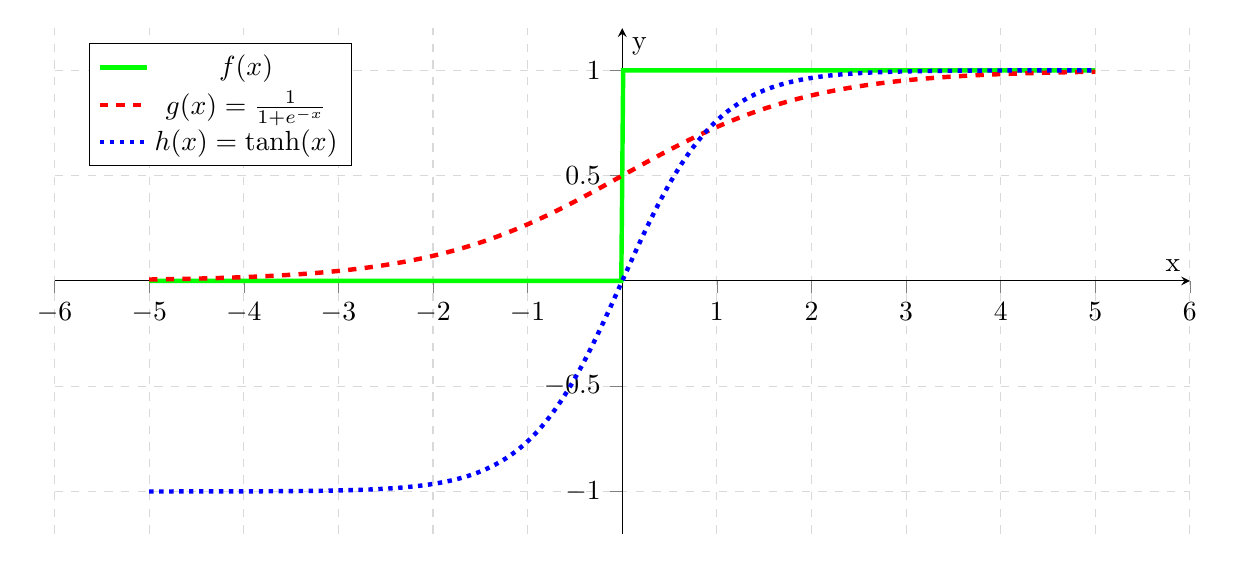
\begin{tikzpicture}[scale=1.0]
        \begin{axis}[
            legend pos=north west,
            axis x line=middle,
            axis y line=middle,
            grid = major,
            width=16cm,
            height=8cm,
            grid style={dashed, gray!30},
            xmin=-5,     % start the diagram at this x-coordinate
            xmax= 5,    % end   the diagram at this x-coordinate
            ymin=-1,     % start the diagram at this y-coordinate
            ymax= 1,   % end   the diagram at this y-coordinate
            %axis background/.style={fill=white},
            xlabel=x,
            ylabel=y,
            tick align=outside,
            enlargelimits=true]
          \addplot[domain=-5:5, green, ultra thick,samples=500] {x < 0 ? 0 : 1};
          \addplot[domain=-5:5, red, ultra thick,samples=500, dashed] {1/(1+exp(-x))};
          \addplot[domain=-5:5, blue, ultra thick,samples=500, dotted] {tanh(x)};
          \addlegendentry{$f(x)$} %TODO: \begin{cases} 0, & x < 0, \\ 1, & x \ge 0, \end{cases} (spacing)
          \addlegendentry{$g(x)=\frac{1}{1+e^{-x}}$}
          \addlegendentry{$h(x)=\tanh(x)$}
        \end{axis} 
    \end{tikzpicture}
    \caption{The unit step function $f$, the sigmoid function $g$ and the hyperbolic tangend $h$.}
    \label{fig:logistic-function}
\end{figure}

\subsection{Unit step function}\label{f:unitstep}
Not so good, because it's not differentiable. Therefore, the backpropagation
algorithm cannot be used.

\subsection{Sigmoid function}\label{f:sigmoid}
Is great because it is infinitely often differentiable.


\subsection{Hyperbolic tangent}\label{f:tanh}
Also differentiable, but gradient descent converges faster (sometimes?)